\section{Blast Algorithm}
\label{sec:blast}

BLAST algorithm is used to search for similar parts of sequence between database and query. There are several implementations of BLAST based on their processing data: nucleotides having 4 letter alphabet and amino acids having 20 letters. The inputs to BLAST are two sequence - database, which consists of a huge amount of data, and a query, which is to be compared with database and find the similar parts of sequence. The output of algorithm are the degree(score) of similarity of the aligned parts and their corresponding location in the sequences. Each of matched pair in database and query is called a High Score Pair(HSP) and is of extreme importance for further biological computations. BLAST algorithm consists of 3 primary steps:
\begin{itemize}
\item{\textit{Pre-processing the query sequence}. The query is divided into several small portions/words.} 
\item{\textit{Searching for the hit}. Obtained small words of query are compared to the data in database to determine the exact match.}
\item{\textit{Expansion of comparison around hits}. In the location where the sequences coincide, the comparison is continued from both sides and HSP is calculated.}
\end{itemize}

\textit{Step 1}. In this step, query is divided into a list of substrings, refer to Fig.\ref{fig:step1}. These substrings are called w-mers of length w \cite{sotiriades2007design}. Let us suppose we have a query DNA sequence ACGTAAARGCAG of length 12 and w-mers of length 3 \cite{sotiriades2007design}. Since the w-mers are contiguous substrings, there are in total 10 w-mers. Indeed, the number of w-mers are calculated as No.of W-mers = [QueryLength - Wmer Length + 1]. The substring ACG will be the first w-mer and CGT is the second and so on. 

\begin{figure}
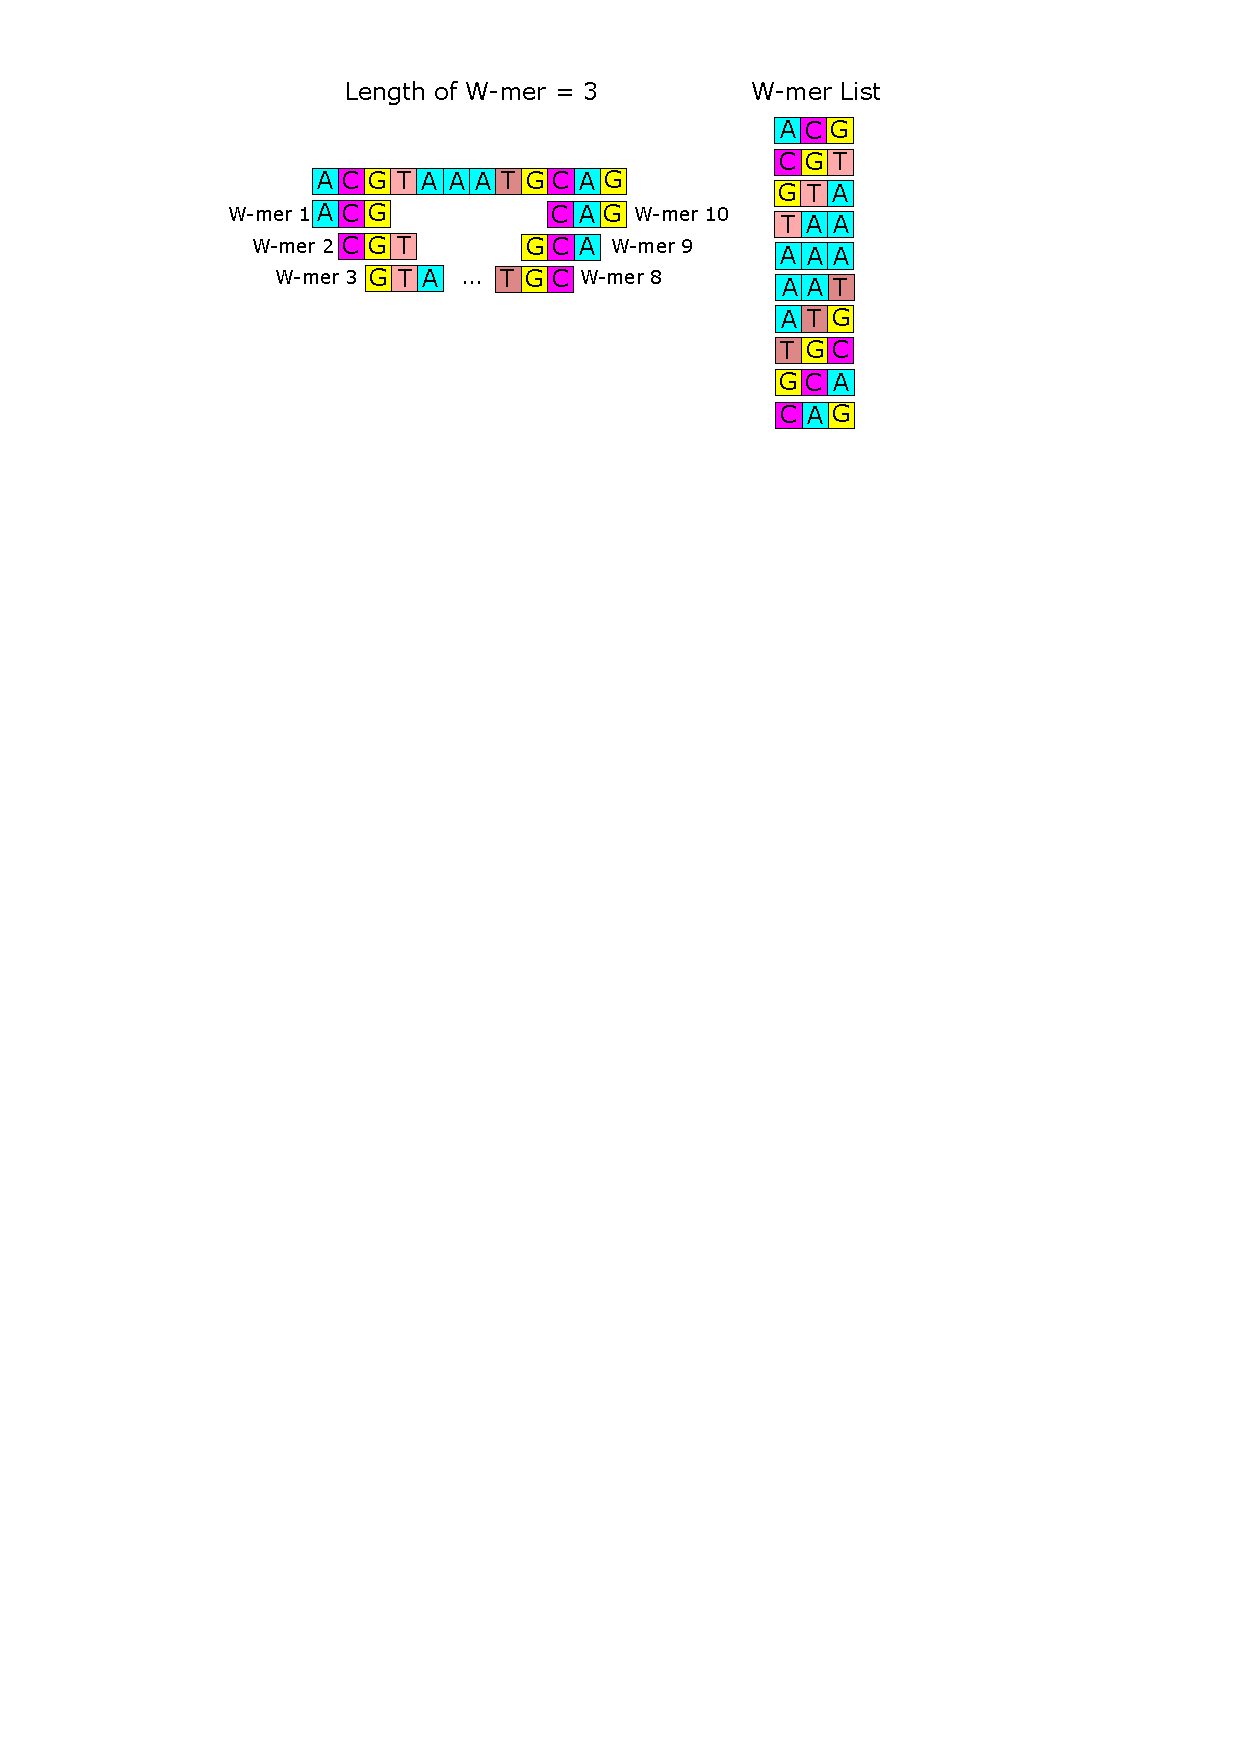
\includegraphics[width=\textwidth]{Figures/Algorithm1.pdf}
\caption{Example of BLAST Algorithm's First Step: Pre-Processing of the Query.} \label{fig:step1}
\end{figure}

\textit{Step 2}. After the query is divided and the list of w-mers is generated, the search for exact match between w-mers and database is conducted. Every found exact match is recorded as a "hit" and saved to proceed further to step 3, refer to Fig\ref{fig:step2}. 

\begin{figure}
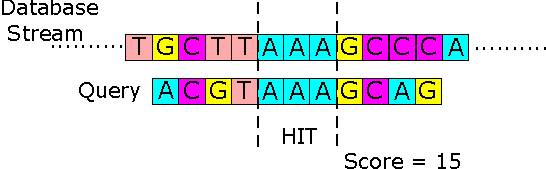
\includegraphics[width=\textwidth]{Figures/Algorithm2.pdf}
\caption{Example of BLAST Algorithm's Second Step: Search for Exact Match/Hit.} \label{fig:step2}
\end{figure}

\textit{Step 3}. After all hits are found, each w-mer/substring is expanded locally to both directions by single letter per direction at a time, refer to Fig\ref{fig:step3}. The expansion holds until the scoring no longer gets improved.
\\

The scoring technique of the algorithm is actually based in the Point Accepted Mutations(PAM) matrices which is used to examine amino-acid "substitutions" are biologically accepted \cite{sotiriades2007design}. However, due to the complexity of this technique, the simpler and biologically acceptable scoring method, that is the result will be correct in biological point of view, will be used. In the expansion stage, each new match will results in addition of 5 and any mismatch will lead to reduction of 4, refer to Fig.\ref{fig:step3}.

\begin{figure}
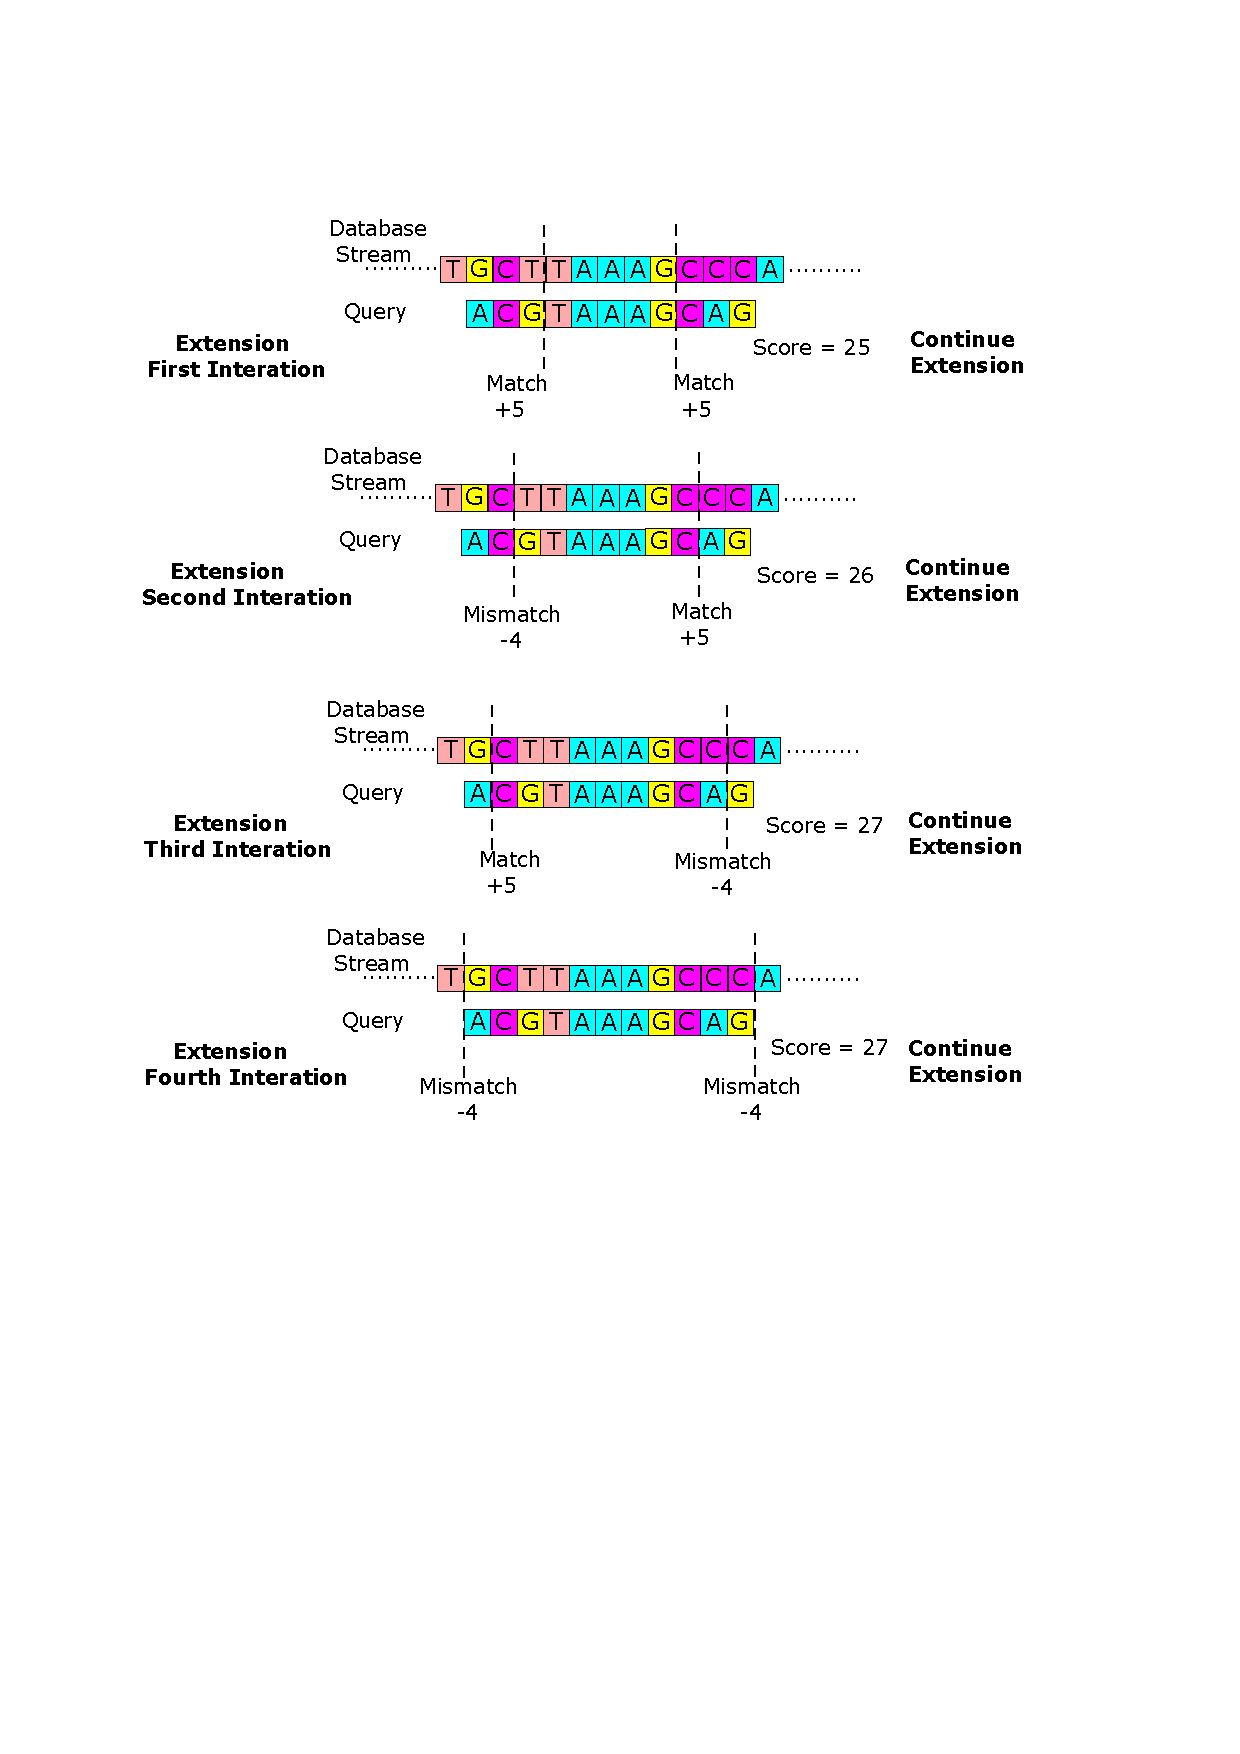
\includegraphics[width=\textwidth]{Figures/Algorithm3.pdf}
\caption{Example of BLAST Algorithm's Third Step: Expansion of Comparison around Hits} \label{fig:step3}
\end{figure}
